\section{Design Example}

\begin{figure}[tb]
\centering
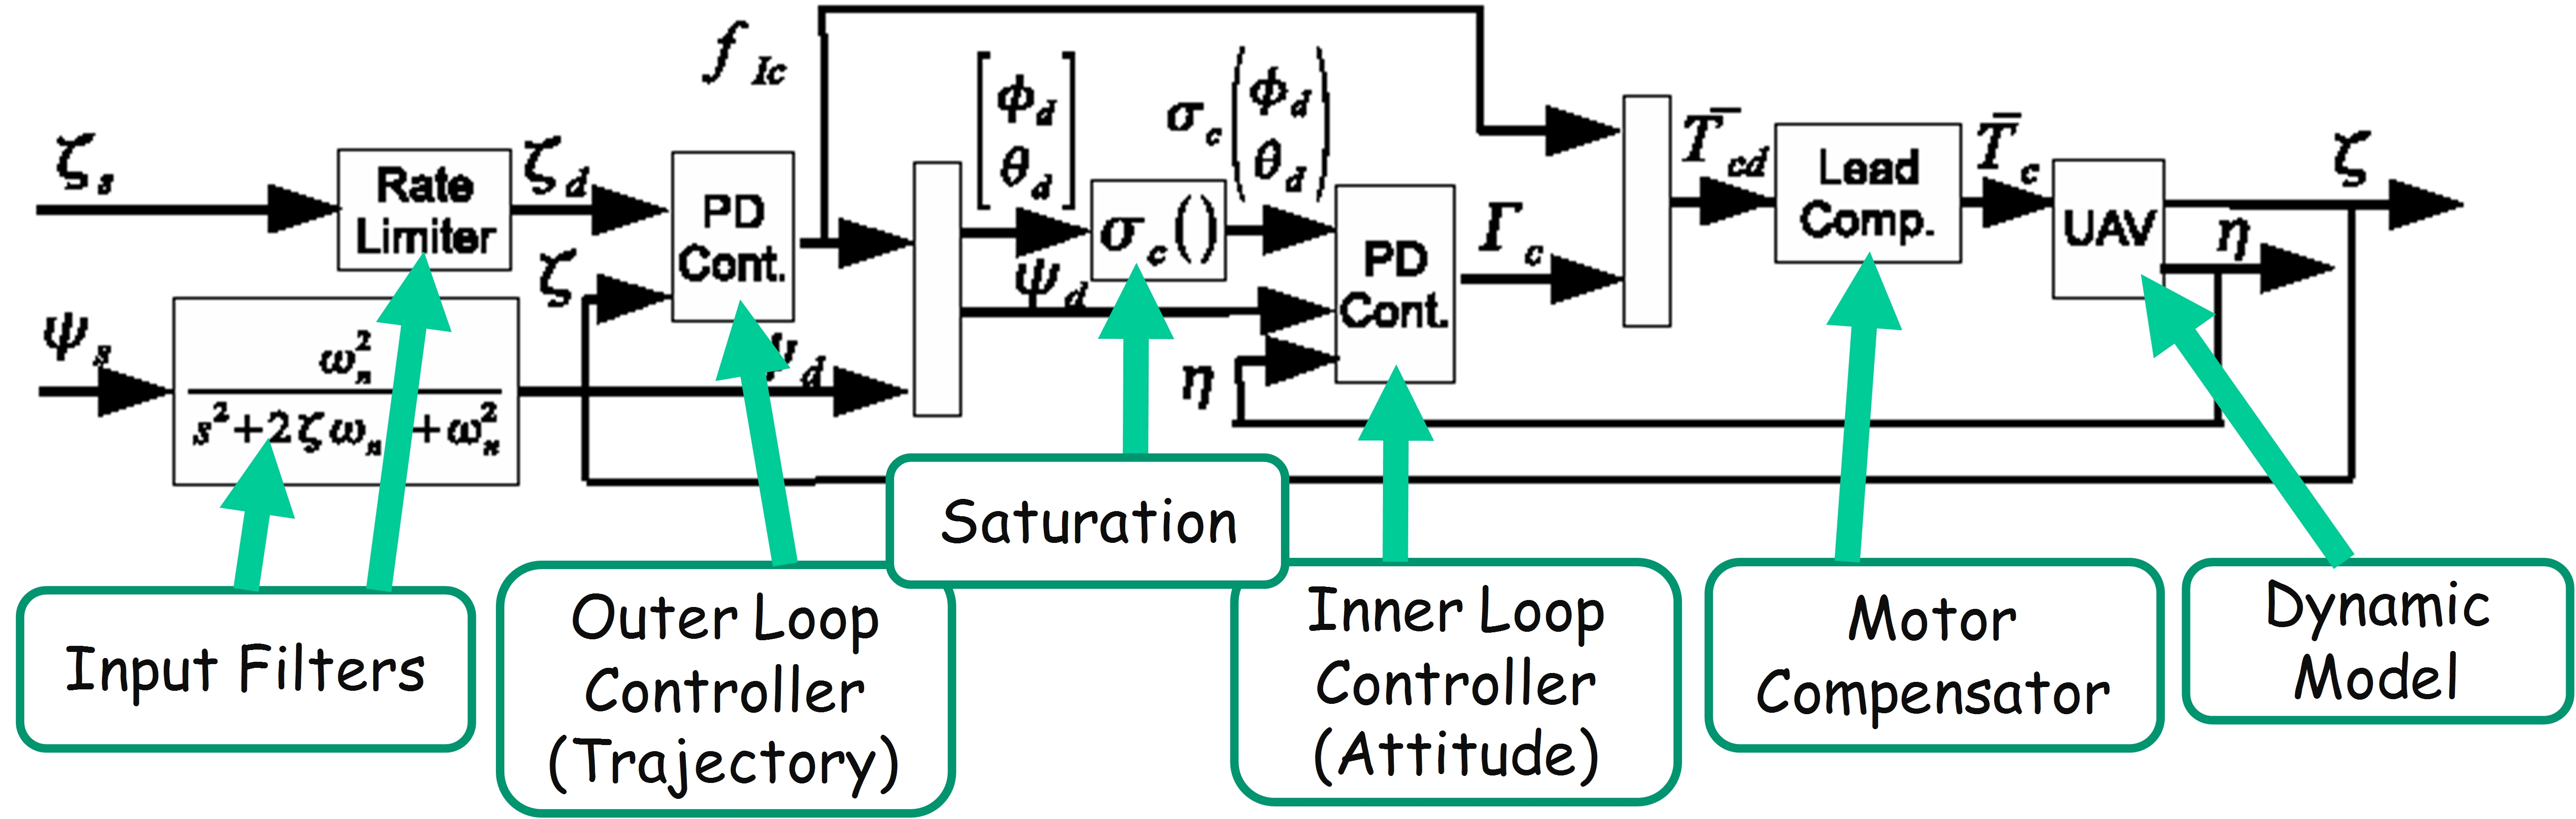
\includegraphics[width=0.85\columnwidth]{figures/quadrotor_arch.png}
    \caption{Basic architecture for the quadrotor control problem.}
    \label{fig:quadrotor}
\end{figure}

Our design example controls a continuous-time system whose model represents a simplified 
version of a quadrotor UAV.  Figure \ref{fig:quadrotor} depicts the basic
component architecture for the control design.  Our example excludes the
nonlinear rotational dynamics of the actual quadrotor for simplicity, but
retains the difficult stability characteristics. Fig. \ref{fig:qr_plant} shows
a Simulink model containing the simplified dynamics. For the fully detailed
quadrotor model and a complete discussion of the control design philosophy, see
\cite{quad:passcontrol}. The example model controls the stack of four
integrators (and motor lag) using two nested PD control loops.
%, as shown in the
%Simulink diagram shown in Fig. \ref{fig:qr_mdl}.  
The Plant block contains the
integrator models. The two control loops (inner and outer, as shown) are
implemented on separate processors, and the execution of the components is
controlled by a simple time-triggered virtual machine that releases tasks and
messages at pre-calculated time instants.

Control design centers around the continuous-time abstraction of passive control \cite{quad:passcontrol}.  
Passivity provides a robust version of continuous-time dynamic stability which is insensitive to 
quantization effects \cite{pass:fettweis86} and network delays \cite{ncs:chopra}\cite{ncs:wireless} 
in digital control implementations.  The passivity conditions help relax constraints on required 
component sample rates, increasing the system's tolerance to jitter and other timing variations. 

Simulated stability analysis yields period parameters for the control components. For 
our discussion the exact nature of these parameters is not important, rather that they represent 
the same behaviors for all of the integrated tools.  Passive design provides a guarantee of stable 
operation around a nominal sampling rate, as the system will tolerate a small number of lost or 
delayed data samples.

% \begin{figure}
% \centering
% 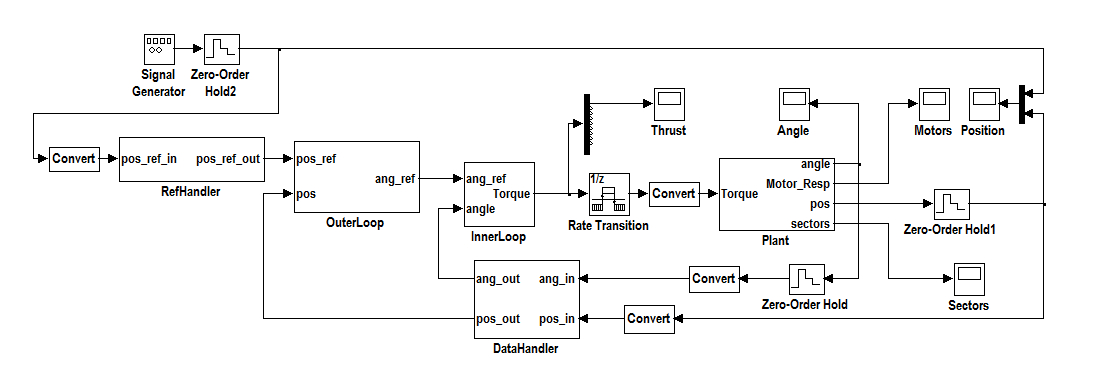
\includegraphics[width=\columnwidth]{figures/quadrotor_mdl.png}
%     \caption{Simulink model of a simplified version of the quadrotor architecture.}
%     \label{fig:qr_mdl}
% \end{figure}

\begin{figure}
\centering
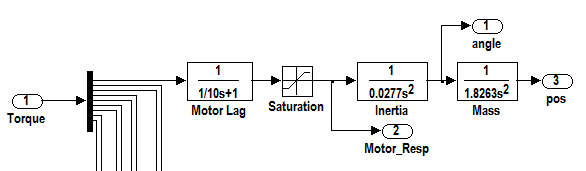
\includegraphics[width=0.9\columnwidth]{figures/quadrotor_plant.png}
    \caption{Simplified quadrotor plant dynamics.  The rotational dynamics have
been removed to facilitate easier study of the behavior.  The full model
includes all of the dynamics.  The signals lines leading off the picture are
signal taps used to perform sector analysis to check stability (see Section 9).}
    \label{fig:qr_plant}
\end{figure}

\begin{figure}
\centering
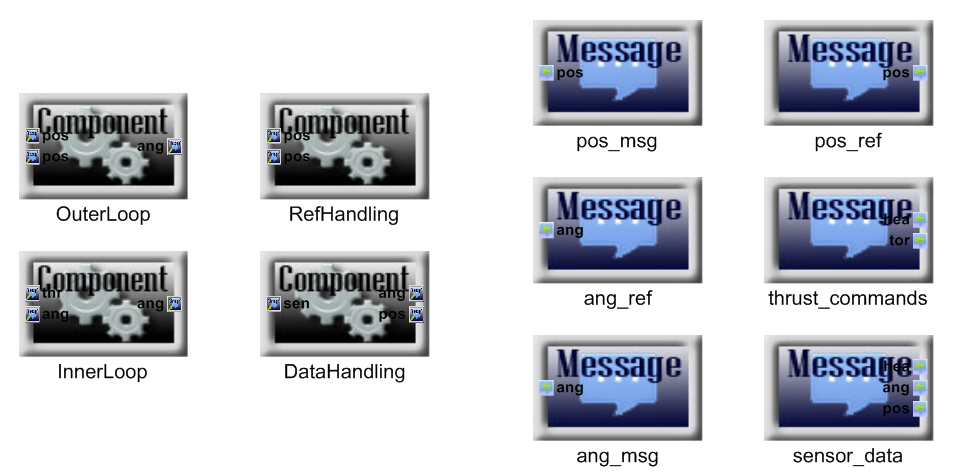
\includegraphics[width=0.9\columnwidth]{figures/quadrotor_types.png}
    \caption{The component type model specifies message types and fields, as well as component types.  Component types specify the mapping of Simulink functional designs to the fields in the messages that will carry the data.  These components and messages are instantiated in the deployment model.}
    \label{fig:qr_types}
\end{figure}

\begin{figure}
\centering
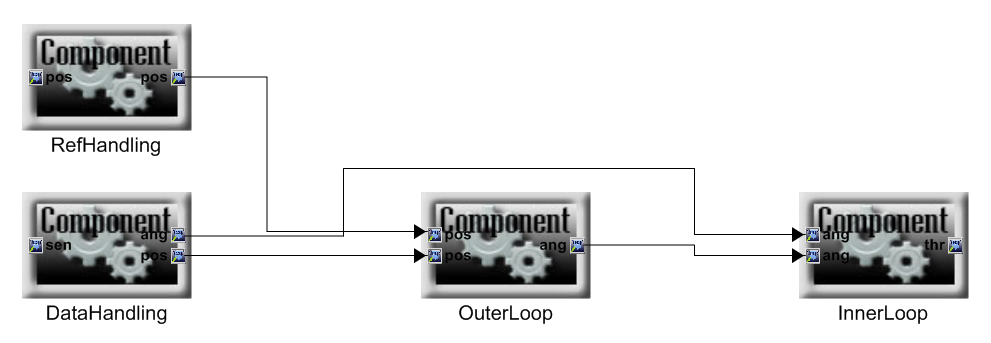
\includegraphics[width=0.9\columnwidth]{figures/quadrotor_log_arch.png}
    \caption{Deployment: The logical architecture model specifies data
dependencies between software component instances. The ports on the blocks
represent data messaging interfaces into and out of the component.}
    \label{fig:qr_log_arch}
\end{figure}

\begin{figure}
\centering
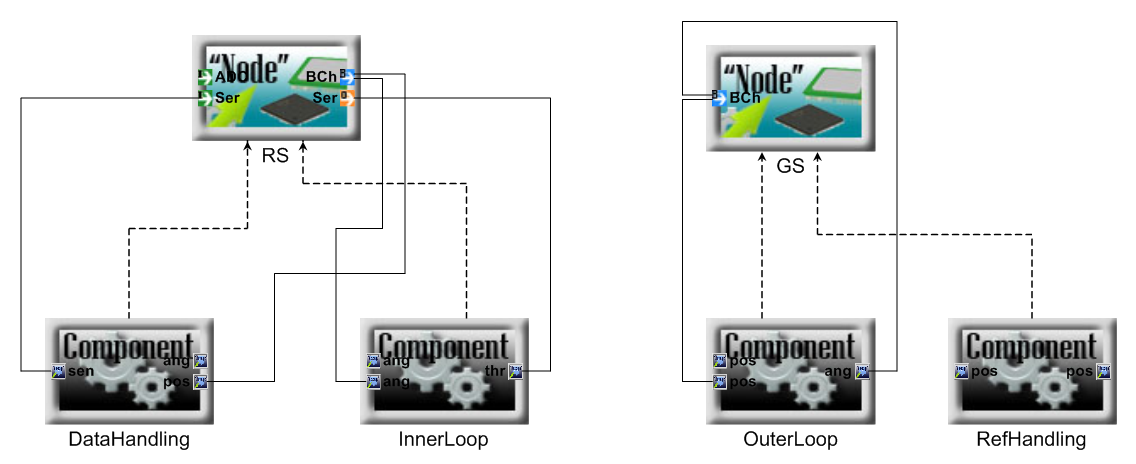
\includegraphics[width=0.9\columnwidth]{figures/quadrotor_hw_mapping.png}
    \caption{Deployment: The platform mapping model specifies the hardware
components that will support the transfer of data to and from each processing
node, the software components that will send and receive the data, and the
message instances in which the data will be carried.  Dashed arrows represent
assignment of components to their respective processor, and solid lines
represent assignment of message instances (component ports) to communication
channels (port objects) on the processor.}
    \label{fig:qr_hw_mapping}
\end{figure}

%\begin{figure}
%\centering
%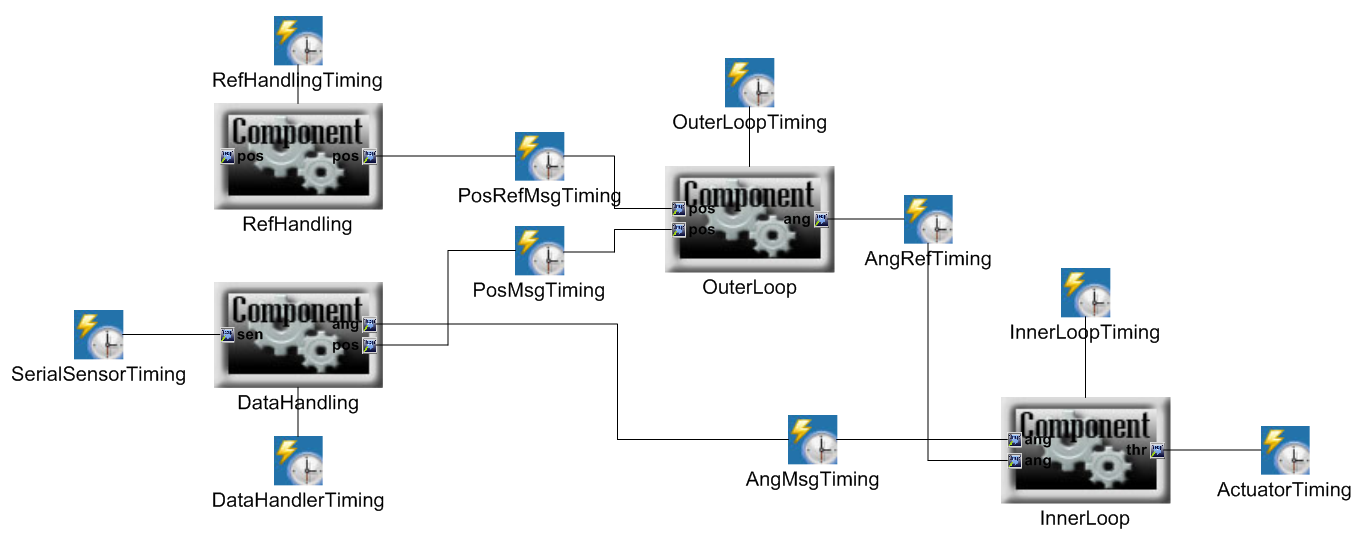
\includegraphics[width=\columnwidth]{figures/quadrotor_timing.png}
%    \caption{Deployment: The execution model indicates which components and
%messages will be scheduled independently.  In the case of
%processor-local data transfers transfer time is neglected, as reads and
%writes occur in locally shared memory.  The locality of a message transfer is
%specified in the architecture and deployment models.  GME provides a separate
%window (not shown) for editing object parameters and attributes.}
%    \label{fig:qr_timing}
%\end{figure}

Figures \ref{fig:qr_types} through \ref{fig:qr_hw_mapping} show different parts of
the GME design model for the quad integrator controller.  The model-integrated
computing approach uses integrated sublanguages to represent models in the
various aspects of the design.

\begin{itemize}
 \item Fig. \ref{fig:qr_types} shows an example of the component typing
language.  Message fields and their sizes are specified here, as well as
component implementations and interfaces.  The quad integrator model has four
different component types (each instantiated once) and six message types
(instantiated as the ports objects appearing on the component instances later
in the design).
 \item Fig. \ref{fig:qr_log_arch} portrays logical data dependencies between
software component instances, independent of their distribution over different
processors.
 \item Fig. \ref{fig:qr_hw_mapping} shows the deployment model -- the mapping
of software components to processing nodes, and data messages to communication
ports.  Two of the four components are mapped to each of the two processors.  RS
(Robostix) is an 8 bit ATMega128 CPU, and GS (Gumstix) is an Intel PXA ARM-based CPU.
% \item Fig. \ref{fig:qr_timing} shows the timing and execution model.  
 \item An execution model (not shown) allows the designer to attach timing parameter
blocks to components and messages.  For the time-triggered case the configuration 
parameters include execution period and worst-case execution time.  The quad integrator
model runs all of the blocks at a frequency of 50Hz.  The execution model also indicates 
which components and messages will be scheduled independently, and which will be
grouped into a single task.  Our example model assigns each component to its own task.
\end{itemize}

Behavior of the deployed components depends on execution timing of the functions
on the platform, the calculated schedule, and coordination between distributed
tasks. The calculated execution schedule can be used to simulate the control
design with additional delays to assess the impact of the platform on
performance.  Fig. \ref{fig:delays} shows simulated effects of additional delays
in the control data paths.  The top of the figure is the direct synchronous
digital implementation of the control system.  The two successive plots show the
effects of adding first one and then two extra delay elements in each control
path.  The reference input frequency and amplitudes were chosen to lie on the
edge of the stable operating point of the design.  This is not meant to be an
exhaustive verification of the control design, rather an illustration of the
gradual oscillation and overshoot degradation that occurs as delays increase.  

\begin{figure}
\centering
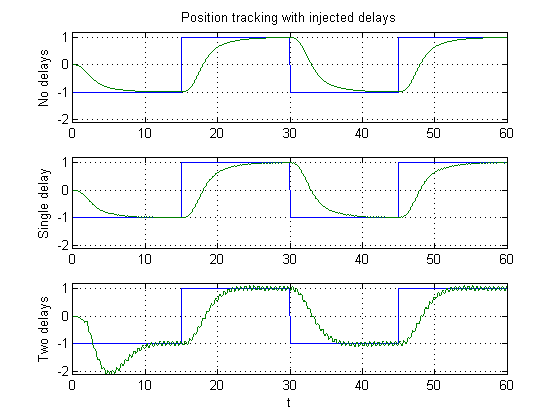
\includegraphics[width=0.9\columnwidth]{figures/delays.png}
    \caption{Effects of increasing delays in the synchronous scheduling of the
control nodes.}
    \label{fig:delays}
\end{figure}

Section 3 discusses our approach to semantic consistency. Sections 4 and 5
cover some details of the model transformations made by the tools to get to
analysis and code artifacts. Sections 6 and 7 briefly describe our approach 
and tools for two of the three semantic models for the language (time-triggered 
scheduling and the execution environment).  Section 8 discusses our approach to 
assessing passivity of the controller, and compares controller performance between 
the simulated design model and the generated controller. Sections 9 and 10 cover 
related work and future work, respectively.  Section 11 concludes.
